\documentclass{beamer}
\newcommand{\m}{\mathcal}
\newcommand{\E}{\mathbb{E}}
\newcommand{\R}{\mathbb{R}}
\mode<presentation>
\usetheme{CambridgeUS}
\title[Stat 992 ]{Predicting Average Medical Payment using Physician Referral Network at the Hospital Service Area Level}
\author{Song Wang, Ruosi Guo, Daniel Ricci 
 }
\date{Nov 10th, 2015}
\begin{document}
\begin{frame}
\titlepage
\end{frame}
\section{Introduction}
\begin{frame}
\frametitle{Background}

\begin{itemize}
 \item {\bf Medicare} In 2012,  covers more than 61 million citizens and used up hundreds of billions years every year.
 \begin{center}
 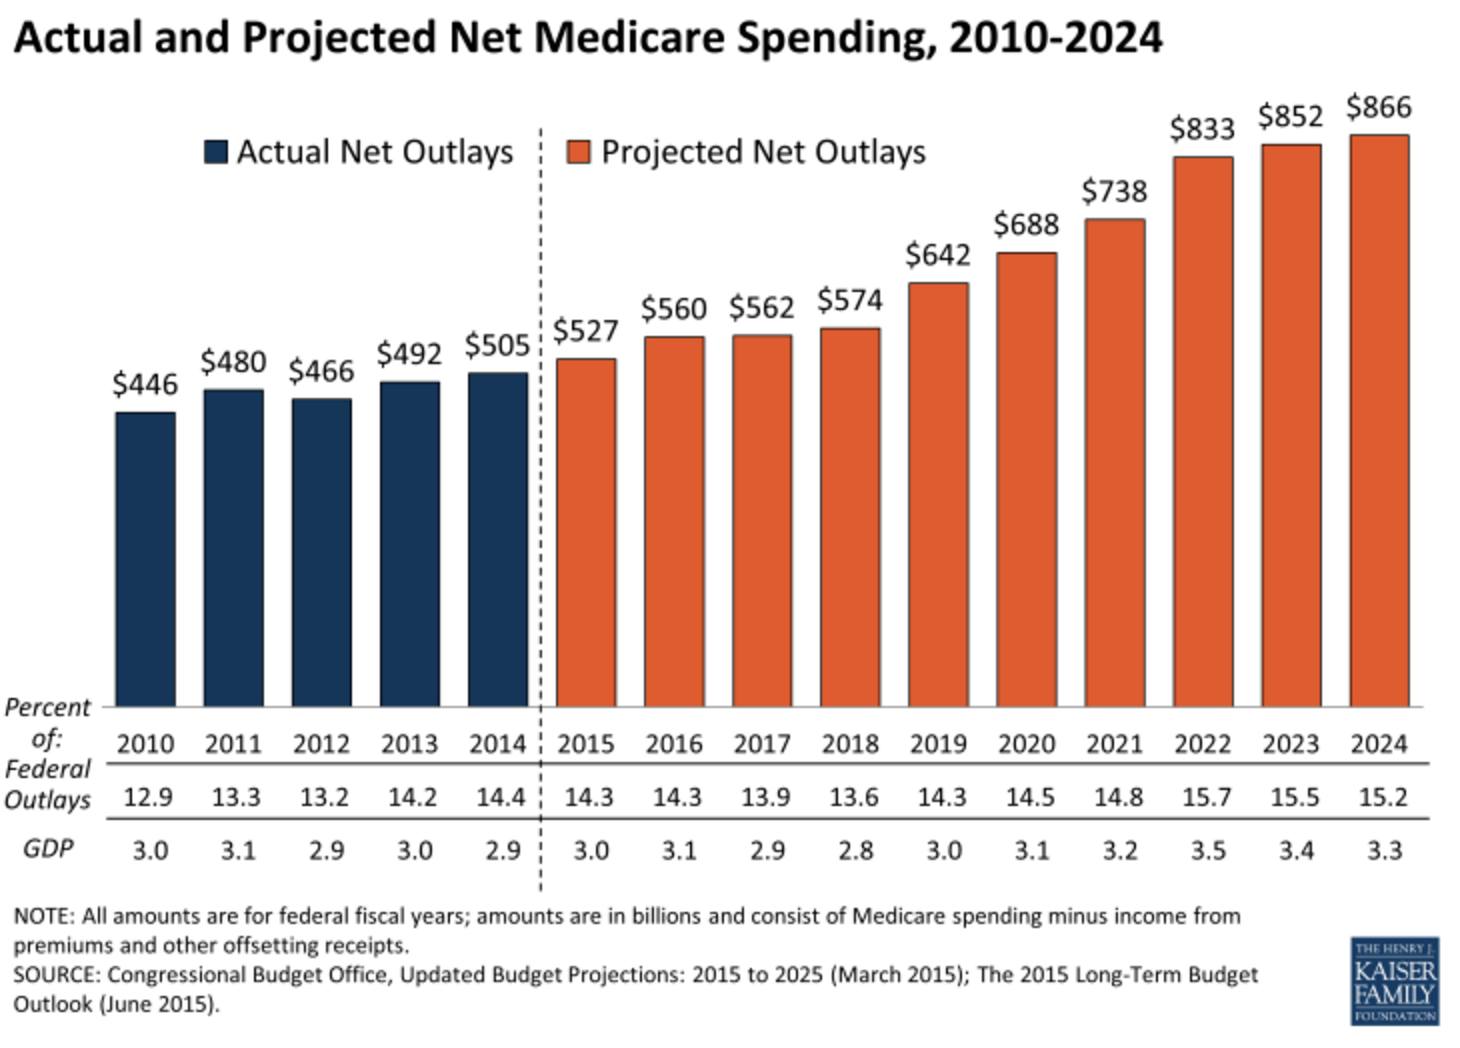
\includegraphics[ width =3in, height =1.22 in] {fig2.png}
 \end{center}
 %\item {\bf Physician referral} is typically frame work for one physician to collaborate and interact with other physicians on patient's care.
\item  {\bf The objective} of our study is to investigate whether there are regional differences in cost of care provided to Medicare Part B beneficiaries, and more specifically, to determine if the cost of care is related to local physician referral network structure. Finally trying to lower the cost medicare.
\end{itemize}
\end{frame}

\begin{frame}
\frametitle{Data sets and Method}
\begin{itemize}
\item Data sets:
\begin{itemize}
\item[-]  Physician referral network 30-day  (2012); 
\item[-]  Hospital Service Areas are collections of zip codes, related covariates corresponding HSA, obtained from dartmouthatlas.org (2012).
\item[-]  Physician Payment Data from CMS (2012)
\end{itemize}
\item Set up \& data pre-processing:
\begin{itemize}
 \item[-] Response Variable:
 average Medicare allowed amount from Payment data, aggregated over the physicians and services in each HSA.
 \item[-] Covariates: -- HSA characteristics, like physician count, resident count, average income, crime rate etc ;\\
    -- Network Characteristics, like mean node degree, edge density, transitivity, closeness etc.
 \end{itemize}
          
\end{itemize}
\end{frame}


\section{Preliminary results}
\subsection{Regression}

\begin{frame}{Results from regression}


\end{frame}


\section{Future Direction}
\begin{frame}
\frametitle{Future directions}
\begin{itemize}
\item Look at some representative networks, explore deeply why and how the physician referral network will affect the cost of Medicare.
\item Build another model based on 2014 data. To see weather there are changes in the regression model and Network  structure.
\end{itemize}

\end{frame}


















\end{document}